\documentclass[a4paper,
  10pt,
  english,
  DIV=12,
  BCOR=8mm]{scrbook}
\usepackage[utf8x]{inputenc}
\usepackage{babel}
\usepackage{listings}
\usepackage{xcolor}
\usepackage{hyperref}
\usepackage{siunitx}
\usepackage[T1]{fontenc}
\usepackage{isodate}
\usepackage{graphicx}
\usepackage{amsthm}
\usepackage{acronym}
\usepackage{amssymb}
\usepackage{tikz}
\usepackage{pgfplots}
\usepackage{caption}
\usepackage{subcaption}
\usepackage{booktabs}
\usepackage{xspace}
\usepackage{overpic}

\bibliographystyle{alpha}

\DeclareSIUnit\byte{B}
\DeclareSIUnit\basepairs{bp}
\DeclareSIUnit\bit{bit}

\definecolor{oceangreen}{cmyk}{1,.0,.20,.78}
\addtokomafont{sectioning}{\rmfamily\color{oceangreen}}

\definecolor{bluekeywords}{rgb}{0.13,0.13,1}
\definecolor{greencomments}{rgb}{0,0.5,0}
\definecolor{turqusnumbers}{rgb}{0.17,0.57,0.69}
\definecolor{redstrings}{rgb}{0.5,0,0}
\definecolor{lightgray}{rgb}{0.9,0.9,0.9}

\usepackage{libertine}
\fontfamily{libertine}
\selectfont
%\usepackage[scaled]{berasans}

\newcommand{\thymine}{\textsc{m}\oldstylenums{2}\xspace}
\newcommand{\local}{\textsc{m}\oldstylenums{1}\xspace}
\newcommand{\algo}[1]{\textsc{{#1}}}
\newcommand{\andi}{\algo{andi}\xspace}
\newcommand{\word}[1]{\textsf{\small#1}}
\newcommand{\wchar}[1]{\textsf{\small#1}}
\newcommand{\eco}{\textsc{eco}\oldstylenums{29}\xspace}
\newcommand{\pneu}{\textsc{Pneu}\oldstylenums{3085}\xspace}

\include{version}

% Todos at the margin
\newcommand{\todo}[1]{
  \marginpar{\fbox{\begin{minipage}{0.9\marginparwidth}
  \scriptsize\sloppy\raggedright #1
  \end{minipage}}}
}


\newtheorem{definition}{Definition}


\lstset{backgroundcolor=\color{lightgray}}

\lstdefinestyle{shell}{
	language=bash,
	columns=flexible,
  xleftmargin=12pt,
  xrightmargin=12pt,
  breaklines=true,
  basicstyle=\small\ttfamily,
  morekeywords={make, tar, git, sudo, andi, time, man, head, cut, fneighbor,
   fretree, figtree, brew, aura, autoreconf},
 % literate={~} {$\sim$}{1}
}

\lstset{style=shell}

\title{Documentation of \algo{andi}}
\subtitle{Rapid Estimation of Evolutionary Distances between Genomes\\ {\small\url{https://github.com/EvolBioInf/andi}}}
\author{Fabian Klötzl\\ \href{mailto:kloetzl@evolbio.mpg.de}{kloetzl@evolbio.mpg.de}}
\date{Version \version, \isodate\today \\
\vspace*{2cm}
\centering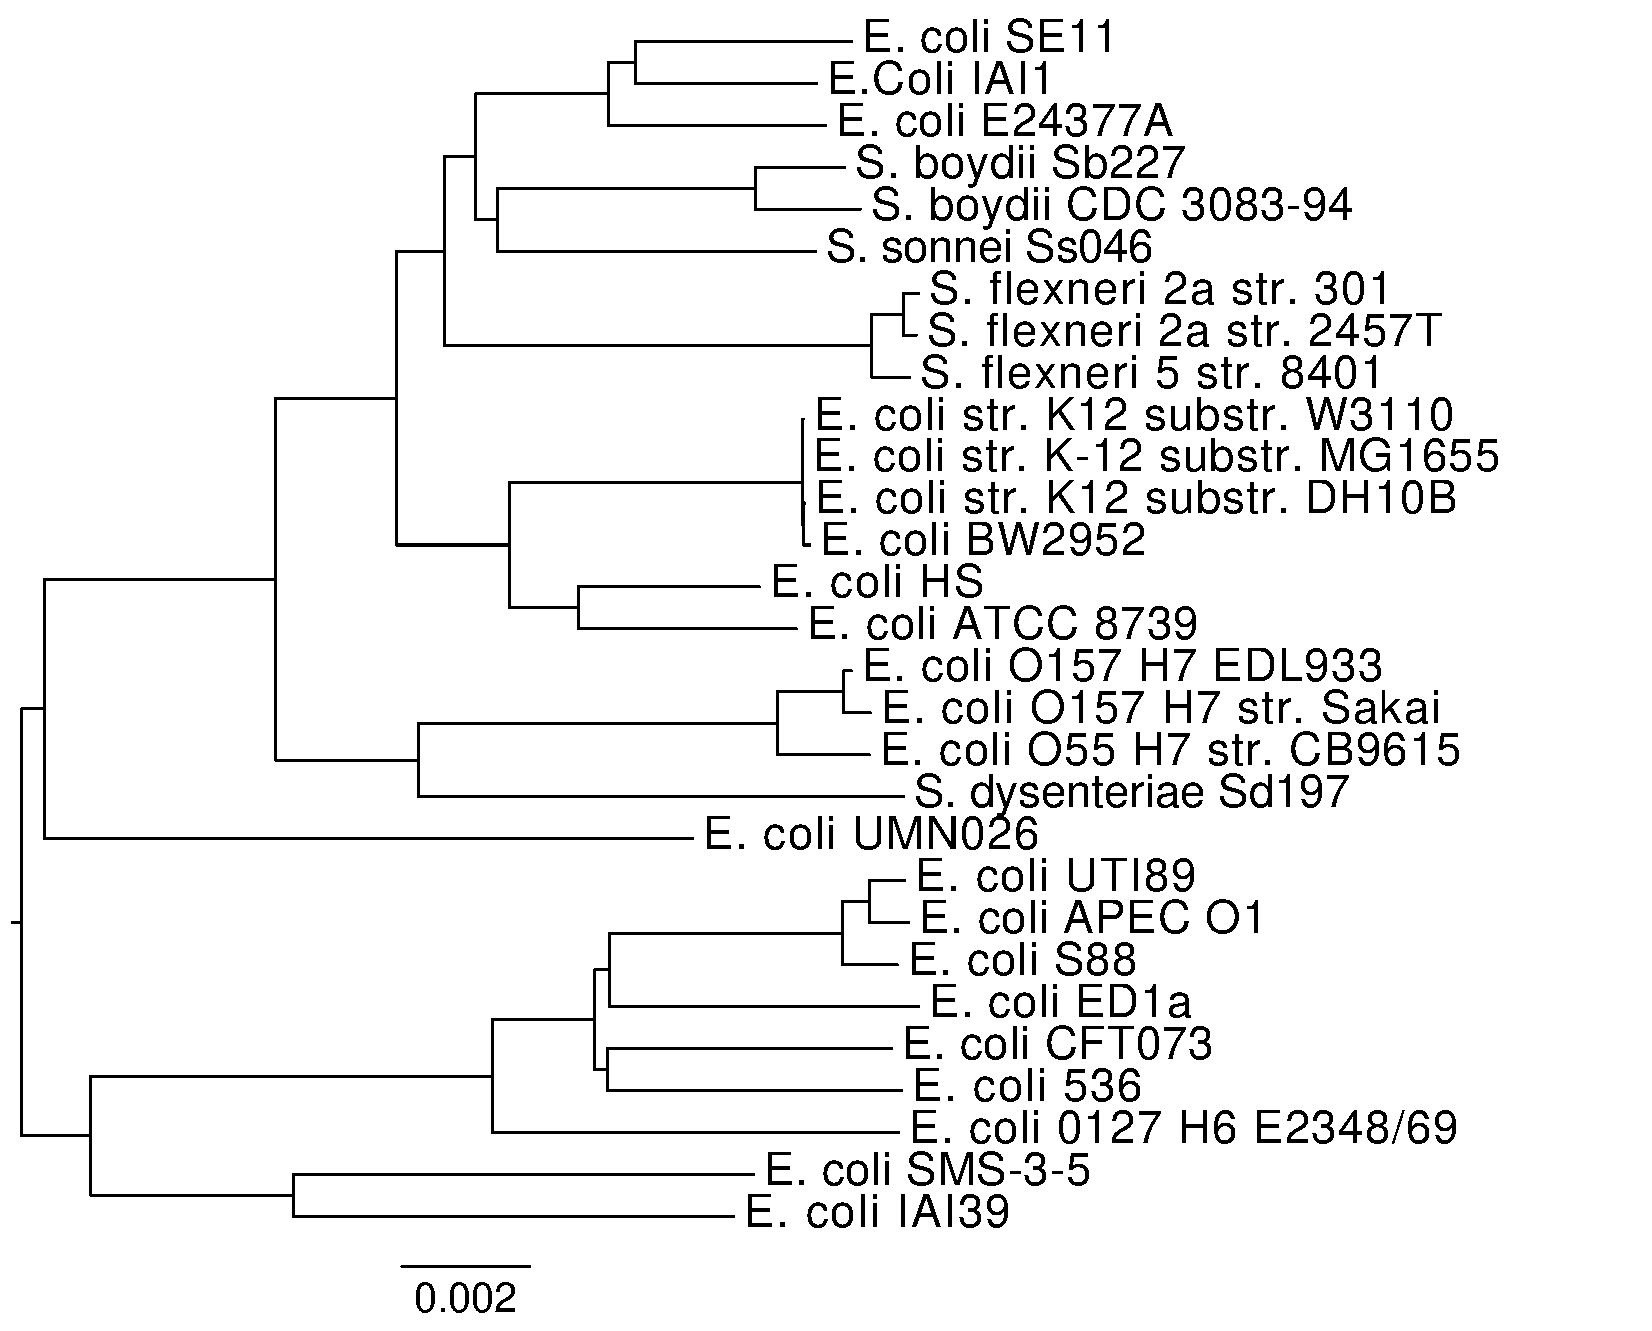
\includegraphics[width=0.8\textwidth]{andi_labels.pdf}}

\begin{document}

\maketitle

\section*{Abstract}
This is the documentation of the \andi program for estimating the evolutionary distance between closely related genomes. These distances can be used to rapidly infer phylogenies for big sets of genomes. Because \andi does not compute full alignments, it is so efficient that it scales well up to thousands of bacterial genomes.

This is scientific software. Please cite our paper \cite{andi} if you use \andi in your publication. Also refer to the paper for the internals of \andi. Additionally, there is a Master's thesis with even more in depth analysis of \andi \cite{kloetzl}.

\vspace*{1cm}
\section*{License}
This document is release under the Creative Commons Attribution Share-Alike license. This means, you are free to copy and redistribute this document. You may even remix, tweak and build upon this document, as long as you credit me for the work I've done and release your document under the identical terms. The full legal code is available online: {\small\url{https://creativecommons.org/licenses/by-sa/4.0/legalcode}}.

\tableofcontents

\chapter{Installation} %%%%%

\section{Package Manager}

The easiest way to install \andi is via a package manager. This also handles all dependencies for you.

\noindent OS X with homebrew:

\begin{lstlisting}
~ %  brew install science/andi
\end{lstlisting}

\noindent ArchLinux:

\begin{lstlisting}
~ %  aura -A andi
\end{lstlisting}

\noindent Debian and Ubuntu (soon):

\begin{lstlisting}
~ %  sudo apt-get install andi
\end{lstlisting}

\andi is intended to run in a \algo{Unix} commandline such as \lstinline$bash$ or \lstinline$zsh$. All examples in this document are also intended for that environment. You can verify that \andi was installed correctly by executing \lstinline$andi -h$. This should give you a list of all available options (see Section~\ref{sec:options}).

\section{Source Package} \label{sub:regular}

Download the latest \href{https://github.com/EvolBioInf/andi/releases}{release} from GitHub. Please note, that \andi requires \algo{libdivsufsort}\footnote{\url{https://github.com/y-256/libdivsufsort}} for optimal performance \cite{divsufsort}. If you wish to install \andi without \algo{libdivsufsort}, consult Section~\ref{sub:wo-divsufsort}.

Once you have downloaded the package, unzip it and change into the newly created directory. 

\begin{lstlisting}
~ %  tar -xzvf andi-0.9.tar.gz
~ %  cd andi-0.9
\end{lstlisting}

\noindent Now build and install \andi.

\begin{lstlisting}
~/andi-0.9 %  ./configure
~/andi-0.9 %  make
~/andi-0.9 %  sudo make install
\end{lstlisting}

\noindent This installs \andi for all users on your system. If you do not have root privileges, you will find a working copy of \andi in the \lstinline$src$ subdirectory. For the rest of this documentation, I will assume, that \andi is in your \textdollar\lstinline!PATH!.

Now \andi should be ready for use. Try invoking the help.

\begin{lstlisting}
~/andi-0.9 %  andi -h
Usage: andi [-jrv] [-p FLOAT] FILES...
	FILES... can be any sequence of FASTA files. If no files are supplied, stdin is used instead.
Options:
  -j, --join        Treat all sequences from one file as a single genome
  -m, --low-memory  Use less memory at the cost of speed
  -p <FLOAT>        Significance of an anchor pair; default: 0.05
  -r, --raw         Calculates raw distances; default: Jukes-Cantor corrected
  -v, --verbose     Prints additional information
  -t <INT>          The number of threads to be used; default: 1
  -h, --help        Display this help and exit
      --version     Output version information and acknowledgments
\end{lstlisting}

\noindent \andi also comes with a man page, which can be accessed via \lstinline$man andi$. % But once you are done with this documentation, you will require it scarcely.

\section{Installing without \algo{libdivsufsort}} \label{sub:wo-divsufsort}

In case you cannot or do not want to install \algo{libdivsufsort}, \andi comes with its own implementation of a \emph{suffix array construction algorithm}. It is called \algo{psufsort} and is also available, separately.\footnote{\url{https://github.com/kloetzl/psufsort}} To activate it for \algo{andi}, proceed as described in Section~\ref{sub:regular}, but with the following twist:

\begin{lstlisting}
~/andi %  ./configure --without-libdivsufsort
\end{lstlisting}

Please note that this requires a C++11 compiler. Also, \algo{psufsort} may be slower than \algo{libdivsufsort} and thus lead to inferior runtimes.

\section{Installing from Git Repository}

To build \andi from the \algo{Git} repo, you will also need the \algo{autotools}. Refer to your OS documentation for installation instructions. Once done, execute the following steps.

\begin{lstlisting}
~ %  git clone git@github.com:EvolBioInf/andi.git
~ %  cd andi
~/andi %  autoreconf -i
\end{lstlisting}

\noindent For old versions of \algo{autoconf} you may instead have to use \lstinline$autoreconf -i -Im4$.

\noindent Continue with the \algo{Gnu} trinity as described in Section~\ref{sub:regular}.


\chapter{Usage} %%%%%

The input sequences for \andi should be in \algo{Fasta} format. Any number of files can be passed. Each file may contain more than one sequence.

\begin{lstlisting}
~ %  andi S1.fasta S2.fasta
2
S1        0.0000 0.0979
S2        0.0979 0.0000
\end{lstlisting}

If no file argument is given, \andi reads the input from \algo{stdin}. This makes it convenient to use in \algo{Unix} pipelines.

\begin{lstlisting}
~ %  cat S1.fasta S2.fasta | andi
2
S1        0.0000 0.0979
S2        0.0979 0.0000
\end{lstlisting}

The output of \andi is a matrix in \algo{Phylip} style: On the first line the number of compared sequences is given, \lstinline!2! in our example. Then the matrix is printed, where each line is preceded by the name of the $i$th sequence. Note that the matrix is symmetric and the main diagonal contains only zeros. The numbers themselves are evolutionary distances, estimated from substitution rates.


\section{Input} \label{sec:join}

As mentioned before, \andi reads in \algo{Fasta} files. It recognizes only the four standard bases and is case insensitive (RegEx: \lstinline![acgtACGT]!). All other residue symbols are excluded from the analysis and \andi prints a warning, when this happens.

If instead of distinct sequences, a \algo{Fasta} file contains contigs belonging to a single taxon, \andi will treat them as a unit when switched into \algo{join} mode. This can be achieved by using the \lstinline!-j! or \lstinline!--join! command line switch.

\begin{lstlisting}
~ %  andi --join E_coli.fasta Shigella.fasta
[Output]
\end{lstlisting}

When the \algo{join} mode is active, the file names are used to label the individual sequences. Thus, in \algo{join} mode, each genome has to be in its own file, and furthermore, at least one filename has to be given via the command line.

If \andi seems to take unusually long, or requires huge amounts of memory, then you might have forgotten the \algo{join} switch. This makes \andi compare each contig instead of each genome, resulting in many more comparisons! To make \andi output the number of genome it about to compare, use the \lstinline$--verbose$ switch.

\section{Output}

The output of \andi is written to \lstinline$stdout$. This makes it easy to use on the command line and within shell scripts. As seen before, the matrix, computed by \algo{andi}, is given in \algo{Phylip} format \cite{phylip}.

\begin{lstlisting}
~ %  cat S1.fasta S2.fasta | andi
2
S1        0.0000 0.0979
S2        0.0979 0.0000
\end{lstlisting}

If the computation completed successfully, \andi exits with the status code 0. Otherwise, the value of \lstinline$errno$ is used as the exit code. \andi can also produce warnings and error messages for the user's convenience. These messages are printed to \lstinline$stderr$ and thus do not interfere with the normal output.

\section{Options} \label{sec:options}

\andi takes a small number of commandline options, of which even fewer are of interest on a day-to-day basis. If \lstinline$andi -h$ displays a \lstinline$-t$ option, then \andi was compiled with multi-threading support (implemented using \algo{OpenMP}). By default \andi uses all available processors. However, to restrict the number of threads, use \lstinline$-t$.

\begin{lstlisting}
~ %  time andi ../test/1M.1.fasta -t 1
2
S1        0.0000 0.0995
S2        0.0995 0.0000
./andi ../test/1M.1.fasta  0,60s user 0,01s system 99% cpu 0,613 total
~ %  time andi ../test/1M.1.fasta -t 2
2
S1        0.0000 0.0995
S2        0.0995 0.0000
./andi ../test/1M.1.fasta -t 2  0,67s user 0,03s system 195% cpu 0,362 total
\end{lstlisting}

In the above examples the runtime dropped from \SI{0.613}{\second}, to \SI{0.362}{\second} using two threads. Giving \andi more threads than input genomes leads to no further speed improvement. \, The other important option is \lstinline$--join$ (see Section~\ref{sec:join}).

By default, the distances computed by \andi are \emph{Jukes-Cantor} corrected \cite{jukescantor}. This means, the output is substitution rates, which is greater than the mismatch rate. To obtain the pure mismatch rate, use the \lstinline$--raw$ switch.

\section{Example: \algo{eco29}}

Here follows a real-world example of how to use \algo{andi}. It makes heavy use of the commandline and tools like \algo{Phylip}. If you prefer \algo{R}, check out this excellent \href{http://holtlab.net/2015/05/08/r-code-to-infer-tree-from-andi-output/}{blog post} by Kathryn Holt.

As a data set we use \algo{eco29}; 29 genomes of \textit{E. Coli} and \textit{Shigella}. You can download the data here: {\small{\url{http://guanine.evolbio.mpg.de/andi/eco29.fasta.gz}}}. The genomes have an average length of 4.9~million nucleotides amounting to a total \SI{138}{\mega\byte}.

\algo{eco29} comes a single \algo{fasta} file, where each sequence is a genome. To calculate their pairwise distances, enter

\begin{lstlisting}
~ % andi eco29.fasta > eco29.mat
andi: The input sequences contained characters other than acgtACGT. These were automatically stripped to ensure correct results.
\end{lstlisting}

\noindent The \algo{eco29} data set includes non-canonical nucleotides, such as \word{Y}, \word{N}, and \word{P}, which get stripped from the input sequences. The resulting matrix is stored in \lstinline$eco29.mat$; Here is a small excerpt:

\begin{lstlisting}
~ % head -n 5 eco29.mat | cut -d ' ' -f 1-5
29
gi|563845 0.0000e+00 1.8388e-02 1.8439e-02 2.6398e-02
gi|342360 1.8388e-02 0.0000e+00 4.4029e-04 2.6166e-02
gi|300439 1.8439e-02 4.4029e-04 0.0000e+00 2.6123e-02
gi|261117 2.6398e-02 2.6166e-02 2.6123e-02 0.0000e+00
\end{lstlisting}

\noindent From this we compute a tree via neighbor-joining using a \algo{Phylip} wrapper called \algo{Embassy}.\footnote{\url{http://emboss.sourceforge.net/embassy/\#PHYLIP}}

\begin{lstlisting}
~ % fneighbor -datafile eco29.mat -outfile eco29.phylipdump
\end{lstlisting}
\noindent To make this tree easier to read, we can midpoint-root it.
\begin{lstlisting}
~ % fretree -spp 29 -intreefile eco29.treefile -outtreefile eco29.tree <<EOF
M
X
Y
R
EOF
\end{lstlisting}

\noindent The file \lstinline$eco29.tree$ now contains the tree in Newick format. This can be plotted using \cite{figtree}

\begin{lstlisting}
~ % figtree eco29.tree &
\end{lstlisting}

\noindent to yield

\begin{figure}[h]
  \centering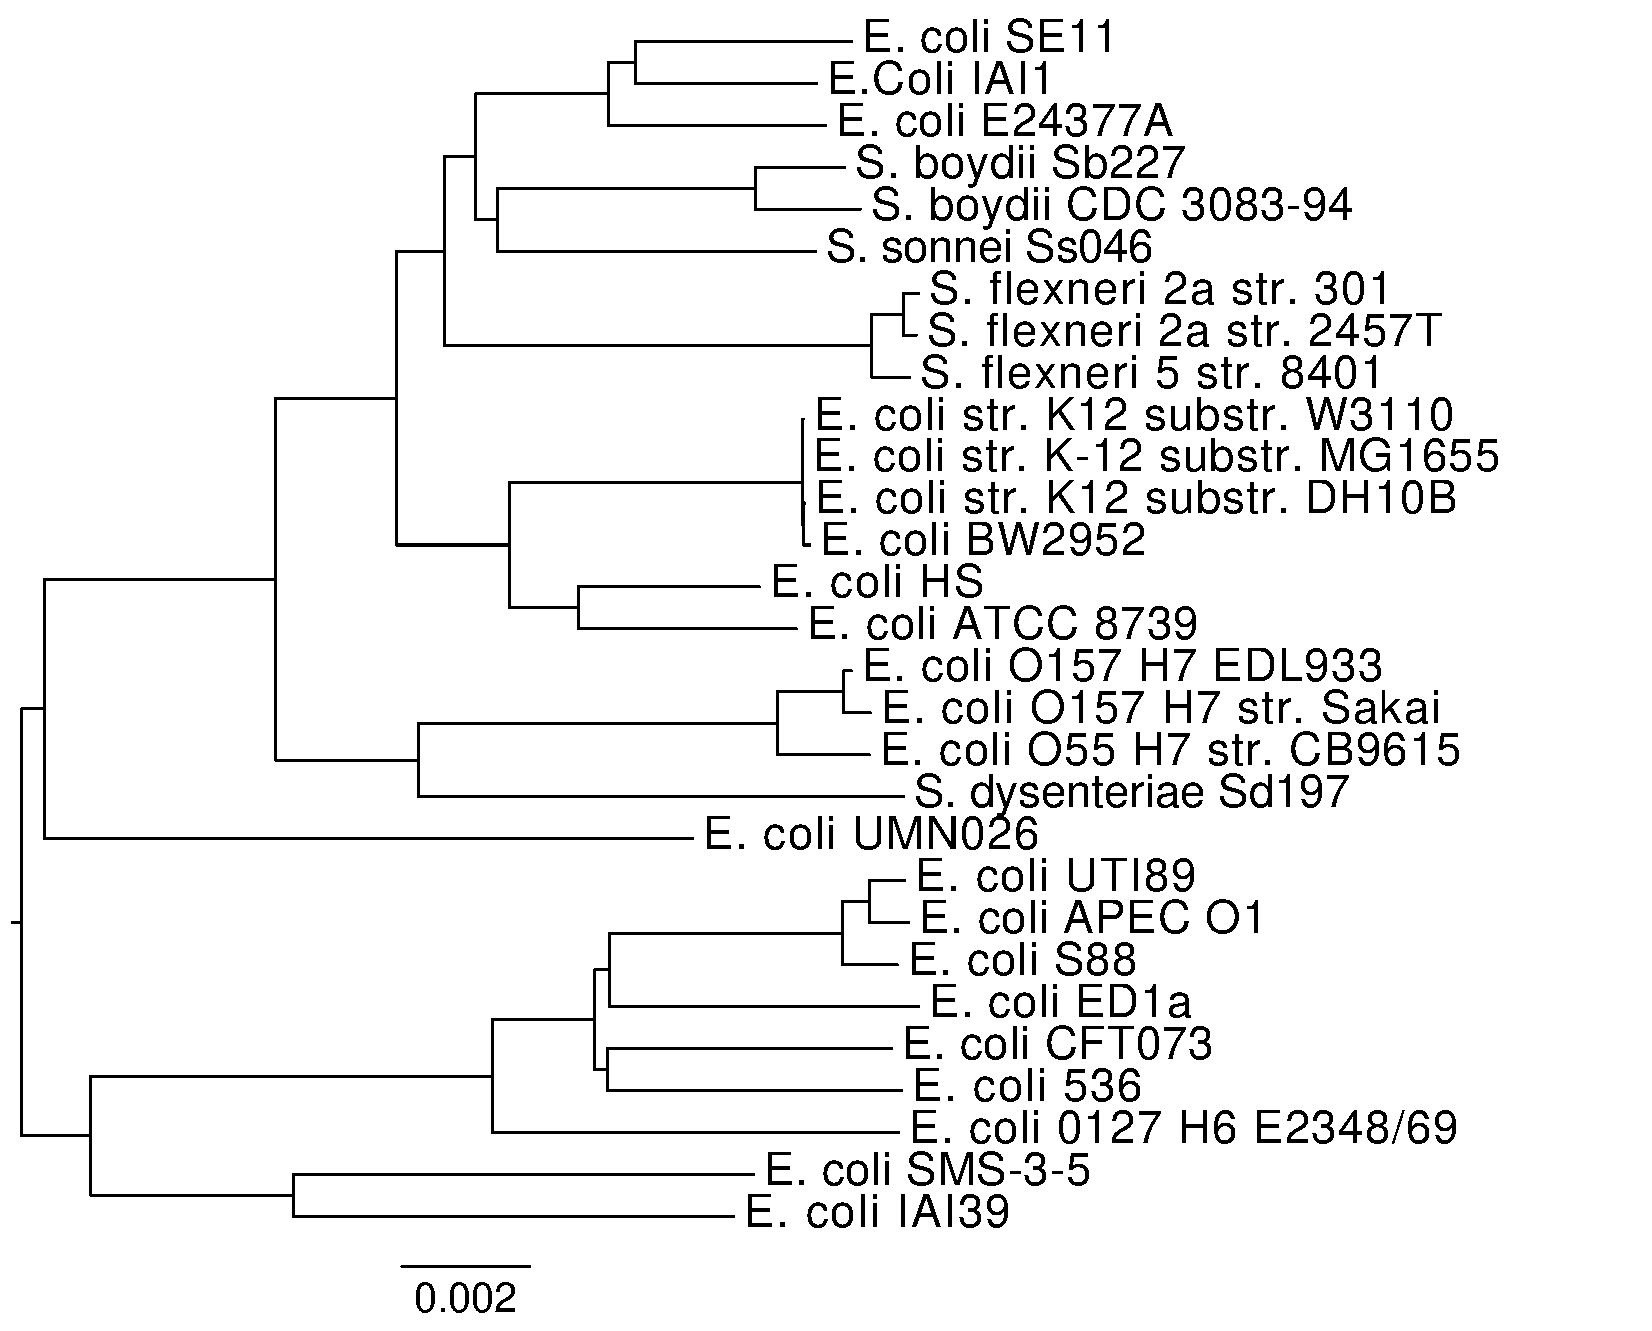
\includegraphics[width=0.8\textwidth]{andi_labels.pdf}
\end{figure}




\chapter{DevOps} %%%%%

\andi is written in C/C++; mostly C99 with some parts in C++11. The sources are released on \algo{GitHub} as \emph{free software} under the \textsc{Gnu General Public License version~3} \cite{GPL}. Prebundled packages using \algo{autoconf} are also available, with the latest release being {\version} at the time of writing.

If you are interested in the internals of \algo{andi}, consult the paper \cite{andi} or my Master's thesis \cite{kloetzl}. Both explain the used approach in detail. The latter emphasizes the used algorithms, data structures and their efficient implementation.

\section{Dependencies}

Here is a complete list of dependencies required for developing \algo{andi}.

\begin{itemize}
  \item A C and a C++11 compiler,
  \item the \algo{autotools},
  \item \algo{Pdflatex} with various packages for the manual,
  \item \algo{Git},
  \item \algo{glib2} for the unit tests,
  \item \algo{doxygen},
  \item and \algo{libdivsufsort}.
\end{itemize}


\section{Code Documentation}

\emph{Every} function in \andi is documented using \algo{doxygen} style comments. To create the documentation run \lstinline$make code-docs$ in the main directory. You will then find the documentation under \lstinline$./docs$.


\section{Unit Tests}

The unit tests are located in the \andi repository under the \lstinline$./test$ directory. Because they require \algo{glib2}, and a C++11 compiler, they are deactivated by default. To enable them, execute

\begin{lstlisting}
~/andi %   ./configure --enable-unit-tests
\end{lstlisting}

\noindent during the installation process. You can then verify the build via 

\begin{lstlisting}
~/andi %   make check
\end{lstlisting}

\noindent The unit tests are also checked each time a commit is sent to the repository. This is done via \algo{TravisCI}.\footnote{\url{https://travis-ci.org/EvolBioInf/andi}} Thus, a warning is produced, when the builds fail, or the unit tests to not run successfully. Currently, the unit tests cover more than 80\% of the code. This is computed via the \algo{Travis} builds and a service called \algo{Coveralls}.\footnote{\url{https://coveralls.io/r/EvolBioInf/andi}}

\section{Known Issues}

These minor issues are known. I intend to fix them, when I have time.

\begin{enumerate}
  \item This code will not work under Windows. At two places Unix-only code is used: filepath-seperators are assumed to be \lstinline$/$ and file-descriptors are used for I/O.
\end{enumerate}


\section{Creating a Release}

A release should be a stable version of \andi with significant improvements over the last version. For bug fixes, dotdot release may be used.

%\subsection{Preparing a new Release}

Once \andi is matured, the new features implemented, and all tests were run, a new release can be created. First, increase the version number in \lstinline$configure.ac$. Commit that change in git, and tag this commit with \lstinline$vX.y$. Create another commit, where you set the version number to the next release (e.\,g., \lstinline$vX.z-beta$). This assures that there is only one commit and build with that specific version. Now return to the previous commit \lstinline$git checkout vX.y$.

Ensure that \andi is ready for packaging with \algo{autoconf}.

\begin{lstlisting}
~ % make distcheck
make  dist-gzip am__post_remove_distdir='@:'
make[1]: Entering directory `/home/kloetzl/Projects/andi'
if test -d "andi-0.9.1-beta"; then find "andi-0.9.1-beta" -type d ! -perm -200 -exec chmod u+w {} ';' && rm -rf "andi-0.9.1-beta" || { sleep 5 && rm -rf "andi-0.9.1-beta"; }; else :; fi
test -d "andi-0.9.1-beta" || mkdir "andi-0.9.1-beta"
 (cd src && make  top_distdir=../andi-0.9.1-beta distdir=../andi-0.9.1-beta/src \
     am__remove_distdir=: am__skip_length_check=: am__skip_mode_fix=: distdir)

... Loads of output ...

=================================================
andi-0.9.1-beta archives ready for distribution: 
andi-0.9.1-beta.tar.gz
=================================================
\end{lstlisting}

If the command does not build successfully, no tarballs will be created. This may necessitate further study of \algo{autoconf} and \algo{automake}. 



\backmatter
%\addcontentsline{toc}{chapter}{Bibliography}
\bibliography{references}

\end{document}
